\documentclass[a4paper,12pt]{article}
\usepackage{amsmath,amsfonts,amssymb} % Math packages
\usepackage{mathtools} % For defining floor and ceiling functions
\usepackage{amsthm}    % Theorems
\usepackage{bm} 	   % Bold math
\usepackage{bbm}	   % More bold math?
\usepackage{array}     % Better tables
\usepackage{chemfig}   % chemical figures
\usepackage{physics}   % derivatives and partials
\usepackage{float}     % Better positioning [H]
\usepackage{framed}    % Framed boxes
\usepackage{geometry}  % Required for adjusting page dimensions and margins
\usepackage{graphicx}  % Include images
\usepackage{multirow}  % multicolumn tables
\usepackage{pgfplots}  % Create plots in latex
\usepackage{siunitx}   % SI unit system
\usepackage{listings}  % Code environments
\usepackage[shortlabels]{enumitem} %lets us change the enumeration to (a), (b), ...
\usepackage{booktabs}  % Better looking horizontal rules
\usepackage{makecell}  % Pre-formatting of column heads
\usepackage{hyperref}  % Clickable links
\renewcommand{\arraystretch}{1.6}

% Theorems and definitions
\theoremstyle{definition}
\newtheorem*{definition}{Definition}
\pgfplotsset{width=10cm,compat=1.9}

% Graph drawings
\usetikzlibrary{shapes,arrows,positioning} % Graph arrows
\usetikzlibrary{automata,positioning,fit,shapes.geometric,backgrounds} % Node grouping

% stats commands
\newcommand{\E}{\mathbb{E}}
\newcommand{\Var}{\mathbb{V}\mathrm{ar}}
\newcommand{\Cov}{\mathbb{C}\mathrm{ov}}
\newcommand{\Risk}{\mathcal{R}}

% common number sets
\newcommand{\N}{\mathbb{N}}
\newcommand{\R}{\mathbb{R}}
\newcommand{\Q}{\mathbb{Q}}
\newcommand{\Z}{\mathbb{Z}}
\newcommand{\C}{\mathbb{C}}

% Cs stuff
\newcommand{\bigO}{\mathcal{O}}

% Indicator function
\newcommand{\Ind}[1]{\mathbbm{1}_{\{#1\}}}

\DeclarePairedDelimiter\ceil{\lceil}{\rceil}
\DeclarePairedDelimiter\floor{\lfloor}{\rfloor}
\DeclarePairedDelimiter\angleb{\langle}{\rangle}

\geometry{
	paper=a4paper, % Paper size, change to letterpaper for US letter size
	top=2.5cm, % Top margin
	bottom=2.5cm, % Bottom margin
	left=2.5cm, % Left margin
	right=2.5cm, % Right margin
	headheight=14pt, % Header height
	footskip=1.5cm, % Space from the bottom margin to the baseline of the footer
	headsep=1.2cm, % Space from the top margin to the baseline of the header
}

\lstset{
	basicstyle=\ttfamily,
	mathescape,
	inputencoding=utf8,
	escapeinside={\%*}{*)},
	literate={á}{{\'a}}1 {ã}{{\~a}}1 {é}{{\'e}}1 {É}{{\'E}}1 {è}{{\`e}}1 {à}{{\`a}}1,
	numbers=left,
	breaklines=true
}

\let\tss\textsuperscript % superscript macro
\let\oldtextbf\textbf
\renewcommand{\textbf}[1]{\oldtextbf{\boldmath #1}}

\newtheorem{exercise}{Exercise}[section]

\begin{document}
\title{Deep Learning}
\author{David Zhao}
\date{Febrary 9, 2023}
\maketitle

\section{Preface}
This paper is a learning documentation adapted from the book \href{https://d2l.ai/}{Dive into Deep learning}.
Coding implementations are omitted.

\section{Preliminaries}
    \subsection*{AutoDifferentiation}

    \subsection*{Linear Algebra}

    \subsection*{Chain Rule}
    Let $y = f(\vec{u})$ such that $\forall i, \vec{u}_i = g_i(\vec{x})$ where $\vec{u} = (u_1, u_2, \ldots, u_m)$ and $\vec{x} = (x_1, x_2, \ldots, x_n)$. \\
    Then
    \begin{equation}
        \begin{aligned}
            \frac{\partial y}{\partial x_i} = \frac{\partial y}{\partial u_1}\frac{\partial u_1}{\partial x_i} + \ldots + \frac{\partial y}{\partial u_m}\frac{\partial u_m}{\partial x_i} 
        \end{aligned}
    \end{equation}

    \subsection*{Baye's Theorem}
    Given any event A and B, 
    \begin{equation}
        \begin{aligned}
            P(A|B) = \frac{P(B|A)P(A)}{P(B)}
        \end{aligned}
    \end{equation}

    \subsection*{Expectations}

\section{Linear Neural Networks for Regression}
    We assume that the relationship between features $\vec{x}$ and target $y$ is approximately linear, i.e,
    \begin{equation}
        E[Y|X=\vec{x}] = x_1w_1 + \ldots + x_dw_d + b \\
    \end{equation}
    where $d$ is the \textit{feature dimensionality}, and $b$ is the \textit{bias}. As such,
    \begin{equation}
        \begin{aligned}
        \hat{y} &= \vec{w}^T\vec{x} + b
                &= X\vec{w} + b
        \end{aligned}
    \end{equation}
    In essence, our goal is to find parameters $\vec{w}$ and $b$ such that our prediction error is 
    minimized for new data examples that are sampled from the same distribution X.

    \subsection*{Loss Function}
    Naturally, our model requires an objective measure of how well or unwell it fits the training data.
    Loss functions fill in this role by quantifying the distance between the \textit{observed} and \textit{predicted}
    labels. The most commonly used loss function is the squared error.
    \begin{equation}
        l^{(i)}(\vec{w},b) = \frac{1}{2}(\hat{y}^{(i)}-\vec{y}^{(i)})^2
    \end{equation}
    Note that the presence of the constant coefficient $\frac{1}{2}$ is notationally convenient as it disappears when we
    take the derivative of the loss function. Also notice that large differences between estimates $\hat{y}^{(i)}$ 
    and targets $\vec{y}^{(i)}$ lead to larger contributions due to the function's quadratic form. In fact, while
    it does encourage our model to avoid sizeable errors, it also yields an excessive sensitivity to anomalous data.
    Finally, to evaluate our model's performance over entire the dataset of $n$ examples, we simply take the average of 
    the losses on the training set:
    \begin{equation}
        L^{(i)}(\vec{w},b) = \frac{1}{n}\sum_{i=1}^{n}\frac{1}{2}(\hat{y}^{(i)}-\vec{y}^{(i)})^2
    \end{equation}
    Hopefully it should be clear by now that our goal is to find parameters $\vec{w}^*$ and $b^*$ such that 
    the total loss is minimized across all examples.

    \subsection*{Minibatch Stochastic Gradient Descent}
    \begin{equation*}
        \begin{aligned}
        (\vec{w},b) &\leftarrow (\vec{w},b) - \frac{\eta}{|\beta|}\sum_{i\in\beta_i}\frac{\partial}{\partial(\vec{w},b)}l^{(i)}(\vec{w},b) \\
        \vec{w}     &\leftarrow \vec{w} - \frac{\eta}{|\beta|}\sum_{i\in\beta_i}\frac{\partial}{\partial\vec{w}}l^{(i)}(\vec{w},b) = \vec{w}- \frac{\eta}{|\beta|}\sum_{i\in\beta_i}\vec{x}^{(i)}(\vec{w}^T\vec{x}^{(i)} + b - \vec{y}^{(i)}) \\
        b           &\leftarrow b - \frac{\eta}{|\beta|}\sum_{i\in\beta_i}\frac{\partial}{\partial b}l^{(i)}(\vec{w},b) = \vec{w}- \frac{\eta}{|\beta|}\sum_{i\in\beta_i}(\vec{w}^T\vec{x}^{(i)} + b - \vec{y}^{(i)})
        \end{aligned}
    \end{equation*}

    \subsection*{Normal Distribution and Squared Loss}
    Recall
    \begin{equation*}
        \begin{aligned}
            p(x) = \frac{1}{\sqrt{2\pi\sigma^2}}\exp({-\frac{1}{2\sigma^2}(x-\mu)^2})
        \end{aligned}
    \end{equation*}
    Assume observations arise from noisy measurements
    \begin{equation*}
        \begin{aligned}
            y = \vec{w}^T\vec{x} + b + \epsilon
        \end{aligned}
    \end{equation*}

    \begin{equation*}
        \begin{aligned}
            p(x) = \frac{1}{\sqrt{2\pi\sigma^2}}\exp({-\frac{1}{2\sigma^2}(y - \vec{w}^T\vec{x} - b)^2})
        \end{aligned}
    \end{equation*}

    \begin{equation*}
        \begin{aligned}
            P(y|X) = \prod_{i=1}^{n}P(\vec{y}^{(i)}|\vec{x}^{(i)})
        \end{aligned}
    \end{equation*}
    since all pairs $(\vec{y}^{(i)},\vec{x}^{(i)})$ were drawn independently. But, maximizing the product of exponential
    functions is tedious. Instead, we minimize the negative log-likelihood:
    \begin{equation*}
        \begin{aligned}
            -\log(y|X) &= -log(\prod_{i=1}^{n}P(\vec{y}^{(i)}|\vec{x}^{(i)})) \\
                       &= \sum_{i=1}^{n} \frac{1}{2}\log(2\pi\sigma^2) + \frac{1}{2\sigma^2}(\vec{y}^{(i)}-\vec{w}^T\vec{x}^{(i)} - b)^2
        \end{aligned}
    \end{equation*}
    As such, it follows that minimizing the square error loss is equivalent to the maximum likelihood estimation of a linear model 
    under additive Gaussian noise.

\subsection*{Generalization}
    The phenomenon of our model fitting closer to the training model than to the underlying distribution is called \textit{overfitting}.
    Instead, our goal is to train our model in such a way that it may find a generalizable pattern and make correct
    predictions about previously unseen data.
    \subsubsection*{Training Error \& Generalization Error}
    In standard supervised learning setting, we assume the training and testing data to be drawn independently from
    identical distributions (i.e. \textit{IID} assumption).
    Training error ($R_{emp}$) is a statistic calculated on the training dataset:
    \begin{equation*}
        \begin{aligned}
           R_{emp}[X,\vec{y},f] = \frac{1}{n}\sum_{i=1}^{n}l(\vec{x}^{(i)},\vec{y}^{(i)},f(\vec{x})^{(i)})
        \end{aligned}
    \end{equation*}
    Generalization error ($R$) is an expectation taken with respect to the underlying distribution:
    \begin{equation*}
        \begin{aligned}
           R[p,f] = E_{(\vec{x},y)\sim P[l(\vec{x},y,f{\vec{x}})]} = \int\int l(\vec{x},y,f(\vec{x}))p(\vec{x},y)d\vec{x}dy
         \end{aligned}
    \end{equation*}
    Note that we can never measure $R$ exactly since the density function $p(\vec{x},y)$ has a form that can almost never
    be precisely known. Moreover, since we cannot sample an infinite stream of data points, we must resort to estimating
    the generalization error by applying our model to an independent test set that is withheld from our training set.
    \subsubsection*{Model Complexity}
    Intuitively, when we have simple models mixed with abundant data, the training and generalization error tend to be close.
    Conversely, we can expect more a complex model and/or fewer examples to cause our training error to diminish, but the
    generalization error to grow. Error on the holdout data, i.e. the validation set, is called the \textit{validation error}.
    
    \subsubsection*{Polynomial Curve Fitting}
    \subsubsection*{Cross Validation}
    In cases when we are dealt with scarce training data, it is likely that we often lack enough hold out data to form a validation
    set. A popular solution is to use \textit{K-fold cross-validation} where the training data is first partitioned into $k$ disjoints 
    sets. Then, we perform a total of $k$ training/validation steps, each time training on $k-1$ sets and validating on the remaining unused set.
    Finally, we average the training and validation errors over the results obtained from our $k$ experiments.
    \subsection*{Weight Decay}
    Recall that we can always mitigate overfitting by collecting more training data. However, gathering more data is often costly, time consuming,
    etc. Therefore, we introduce our first \textit{regularization} technique known as \textit{weight decay}.
    
    Note that we may also limit model complexity by tweaking the degree of our fitted polynomial. However, even small
    changes in degree can dramatically increase model complexity, hence motivating our necessity for a more fine-tuning method, i.e. weight decay.

    \subsubsection*{Norms \& Weight Decay}
    \begin{equation*}
        \begin{aligned}
            \vec{w}     &\leftarrow (1-\eta\lambda)\vec{w} - \frac{\eta}{|\beta|}\sum_{i\in\beta_i}\frac{\partial}{\partial\vec{w}}l^{(i)}(\vec{w},b) = \vec{w}- \frac{\eta}{|\beta|}\sum_{i\in\beta_i}\vec{x}^{(i)}(\vec{w}^T\vec{x}^{(i)} + b - \vec{y}^{(i)}) \\
        \end{aligned}
    \end{equation*}

\section{Linear Neural Networks for Classification}
    \subsection*{Softmax Regression}


    \begin{equation*}
        \begin{aligned}
             = \hat{y}_i = \frac{\exp(o_i)}{\sum_{j}\exp(o_j)}
        \end{aligned}
    \end{equation*}
    
\section{Multilayer Perceptrons}
Recall in section 3, we described affine transformations as linear transformations with added bias. This model maps inputs directly to
outputs via a single affine transformation, followed by a softmax operation. However, linearity is often a strong assumption.
    \subsection*{Limitations of Linear Models}
    Linearity implies the weaker law of \textit{monotonicity} i.e. any increase in inputs must always correspond to an increase in our model's 
    output (positive weights), or a decrease in our model's output (negative weights). Often times, linearity becomes too strong of an assumption
    to be applied to problems that require more specific modelling. Suppose for example we want to predict whether an individual will repay loan
    based on their salary. Though monotonic, this relationship is perhaps not linear as an increase in income from \$0 to \$50,000 likely
    corresponds to a higher likelihood of repayment than an increase from \$1 million to \$1.05 million. As such, it may be preferable to
    post-process our outcome by using a logarithmic map, to make linearity more plausible.
    \subsection*{Incorporating Hidden Layers}
    We overcome the limitations of linearity by incorporating one or more hidden layers. The most common way to do this is to stack many fully
    connected layers on top of each other. We can think of the first $L-1$ layers as our representation and the final layer as our linear predictor.
    This architecture is commonly called a \textit{multilayer preceptron} or \textit{MLP}.

    \subsection*{From Linear to Nonlinear}
    \begin{figure}[h]
        \centering
        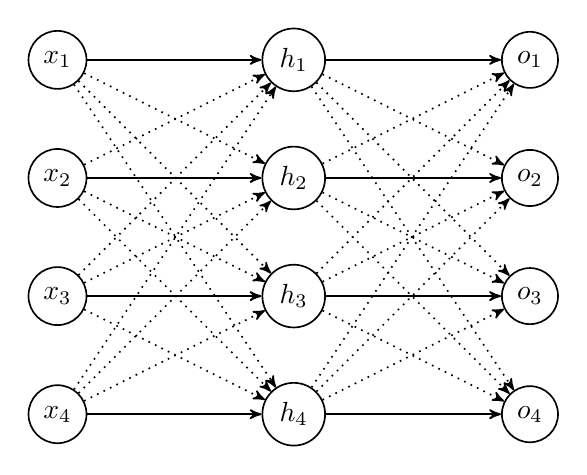
\begin{tikzpicture}[->, >=stealth', auto, semithick, node distance=3cm]
        \tikzstyle{every state}=[fill=white,draw=black,thick,text=black,scale=1]
        \node[draw, circle]    (x1) at (0,0)        {$x_1$};
        \node[draw, circle]    (x2) at (0,-1.5)     {$x_2$};
        \node[draw, circle]    (x3) at (0,-3)       {$x_3$};
        \node[draw, circle]    (x4) at (0,-4.5)     {$x_4$};
        \node[draw, circle]    (h1) at (3,0)        {$h_1$};
        \node[draw, circle]    (h2) at (3,-1.5)     {$h_2$};
        \node[draw, circle]    (h3) at (3,-3)       {$h_3$};
        \node[draw, circle]    (h4) at (3,-4.5)     {$h_4$};
        \node[draw, circle]    (o1) at (6,0)        {$o_1$};
        \node[draw, circle]    (o2) at (6,-1.5)     {$o_2$};
        \node[draw, circle]    (o3) at (6,-3)       {$o_3$};
        \node[draw, circle]    (o4) at (6,-4.5)     {$o_4$};
        \begin{scope}[on background layer]
        \end{scope}
        \path
        (x1) edge[]	node{}	        (h1)
        (x1) edge[dotted]	node{}	(h2)
        (x1) edge[dotted]	node{}	(h3)
        (x1) edge[dotted]	node{}	(h4)
        (x2) edge[dotted]	node{}	(h1)
        (x2) edge[]	node{}	        (h2)
        (x2) edge[dotted]	node{}	(h3)
        (x2) edge[dotted]	node{}	(h4)
        (x3) edge[dotted]	node{}	(h1)
        (x3) edge[dotted]	node{}	(h2)
        (x3) edge[]	node{}	        (h3)
        (x3) edge[dotted]	node{}	(h4)
        (x4) edge[dotted]	node{}	(h1)
        (x4) edge[dotted]	node{}	(h2)
        (x4) edge[dotted]	node{}	(h3)
        (x4) edge[]	node{}	        (h4)
        (h1) edge[]	node{}	        (o1)
        (h1) edge[dotted]	node{}	(o2)
        (h1) edge[dotted]	node{}	(o3)
        (h1) edge[dotted]	node{}	(o4)
        (h2) edge[dotted]	node{}	(o1)
        (h2) edge[]	node{}	        (o2)
        (h2) edge[dotted]	node{}	(o3)
        (h2) edge[dotted]	node{}	(o4)
        (h3) edge[dotted]	node{}	(o1)
        (h3) edge[dotted]	node{}	(o2)
        (h3) edge[]	node{}	        (o3)
        (h3) edge[dotted]	node{}	(o4)
        (h4) edge[dotted]	node{}	(o1)
        (h4) edge[dotted]	node{}	(o2)
        (h4) edge[dotted]	node{}	(o3)
        (h4) edge[]	node{}	        (o4);
        \end{tikzpicture}
        \caption{An MLP with a hidden layer of 4 hidden units.}
      \end{figure}
    \subsection*{Activation Functions}
    \subsubsection*{ReLU Function}
    The most popular choice, due to both simplicity of implementation and its good performance on a variety of predictive tasks, is the rectified linear unit (ReLU) 
    ReLU provides a very simple nonlinear transformation. Given an element $x$, the function is defined as the maximum of that element and 0:
    \begin{equation*}
        \begin{aligned}
            ReLU(x) = \max(x,0)
        \end{aligned}
    \end{equation*}
    When the input is negative, the derivative of the ReLU function is 0, and when the input is positive, the derivative of the ReLU function is 1. Note that the ReLU 
    function is not differentiable when the input takes value precisely equal to 0. In these cases, we default to the left-hand-side derivative and say that the derivative
    is 0 when the input is 0.
    \subsubsection*{Sigmoid Function}
    \begin{equation*}
        \begin{aligned}
            sigmoid(x) = \frac{1}{1+\exp(-x)}
        \end{aligned}
    \end{equation*}
    \subsubsection*{Tanh Function}
    \begin{equation*}
        \begin{aligned}
            tanh(x) = \frac{1-\exp(-2x)}{1+\exp(-2x)}
        \end{aligned}
    \end{equation*}

    Variational autoencoders
    Standard distribution
    non-standard distribution gaussian
    What is the difference between 
    why do we initialize parameters with gaussian noise
    How are activation fuctions used
\end{document}